
\chapter*{Preface}
\markright{}
\addcontentsline{toc}{section}{Preface}

% Position the image to the right of the heading.
\vspace{-7\baselineskip} % move up
\hfill
 \begin{minipage}{0.5\textwidth}
 \centering
 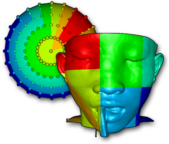
\includegraphics{VTKTextbook-6}
 % \captionof*{figure}{\textit{}}
 \end{minipage}
\vspace{2\baselineskip}


\firstletter{V}isualization is a great field to work in these days. Advances in computer hardware and software have brought this technology into the reach of nearly every computer system. Even the ubiquitous personal computer now offers specialized 3D graphics hardware at discount prices. And with recent releases of the Windows operating systems such as XP, OpenGL has become the de facto standard API for 3D graphics.

 We view visualization and visual computing as nothing less than a new form of communication. All of us have long known the power of images to convey information, ideas, and feelings. Recent trends have brought us 2D images and graphics as evidenced by the variety of graphical user interfaces and business plotting software. But 3D images have been used sparingly, and often by specialists using specialized systems. Now this is changing. We believe we are entering a new era where 3D images, visualizations, and animations will begin to extend, and in some cases, replace the current communication paradigm based on words, mathematical symbols, and 2D images. Our hope is that along the way the human imagination will be freed like never before.

This text and companion software offers one view of visualization. The field is broad, including elements of computer graphics, imaging, computer science, computational geometry, numerical analysis, statistical methods, data analysis, and studies in human perception. We certainly do not pretend to cover the field in its entirety. However, we feel that this text does offer you a great opportunity to learn about the fundamentals of visualization. Not only can you learn from the written word and companion images, but the included software will allow you to \textit{practice} visualization. You can start by using the sample data we have provided here, and then move on to your own data and applications. We believe that you will soon appreciate visualization as much as we do.

In this, the third edition of \textit{Visualization Toolkit} textbook, we have added several new features since the first and second editions. Volume rendering is now extensively supported, including the ability to combine opaque surface graphics with volumes. We have added an extensive image processing pipeline that integrates conventional 3D visualization and graphics with imaging. Besides several new filters such as clipping, smoothing, 2D/3D Delaunay triangulation, and new decimation algorithms, we have added several readers and writers, and better support net-based tools such as Java and VRML. VTK now supports cell attributes, and attributes have been generalized into data arrays that are labeled as being scalars, vectors, and so on. Parallel processing, both shared-memory and distributed models, is a major addition. For example, VTK has been used on a large 1024--processor computer at the US National Labs to process nearly a petabyta of data. A suite of 3D widgets is now available in VTK, enabling powerful data interaction techniques. Finally, VTK's cross-platform support has greatly improved with the addition of CMake---a very nice tool for managing the compile process (\href{https://www.cmake.org}{https://www.cmake.org}).

The additions of these features required the support of three special contributors to the text: Lisa Sobierajski Avila, Rick Avila, and C. Charles Law. Rick and Lisa worked hard to create an object-oriented design for volume rendering, and to insure that the design and software is fully compatible with the surface-based rendering system. Charles is the principle architect and implementer for the imaging pipeline. We are proud of the streaming and caching capability of the architecture: It allows us to handle large data sets despite limited memory resources.

Especially satisfying has been the response from users of the text and software. Not only have we received a warm welcome from these wonderful people, but many of them have contributed code, bug fixes, data, and ideas that greatly improved the system. In fact, it would be best to categorize these people as co--developers rather than users of the system. We would like to encourage anyone else who is interested in sharing their ideas, code, or data to contact the VTK user community at \href{https://www.vtk.org/}{https://www.vtk.org/}, or one of the authors. We would very much welcome any contributions you have to make. Contact us at \href{https://www.kitware.com/}{https://www.kitware.com/}\index{Kitware, Inc.!www.kitware.com}. We also provide commercial support\index{Kitware, Inc.!VTK commercial support}.

This edition is based on the fourth edition. It differs in that the PDF versionis extensively cross--referenced and indexed. Also, where possible, equations and figures have been updated. Figures that exist as VTK examples are linked to the nightly output of the regression testing.

\chapter*{Acknowledgments}
\markright{}
\addcontentsline{toc}{section}{Acknowledgments}

% Position the image to the right of the heading.
\vspace{-7\baselineskip} % move up
\hfill
 \begin{minipage}{0.5\textwidth}
 \centering
 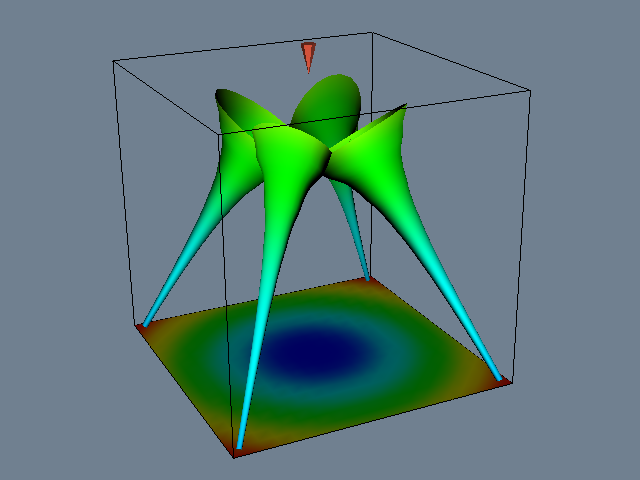
\includegraphics[width=0.98\textwidth]{Figure9-15}
 % \captionof*{figure}{\textit{}}
 \end{minipage}
\vspace{2\baselineskip}



\firstletter{D}uring the creation of the \textit{Visualization Toolkit} we were fortunate to have the help of many people. Without their aid this book and the associated software might never have existed. Their contributions included performing book reviews, discussing software ideas, creating a supportive environment, and providing key suggestions for some of our algorithms and software implementations.

We would like to first thank our management at the General Electric Corporate R\&D Center who allowed us to pursue this project and utilize company facilities: Peter Meenan, Manager of the Computer Graphics and Systems Program, and Kirby Vosburgh, Manager of the Electronic Systems Laboratory. We would also like to thank management at GE Medical Systems who worked with us on the public versus proprietary software issues: John Lalonde, John Heinen, and Steve Roehm.

We thank our co-workers at the R\&D Center who have all been supportive: Matt Turek, for proof reading much of the second edition; also Majeid Alyassin, Russell Blue, Jeanette Bruno, Shane Chang, Nelson Corby, Rich Hammond, Margaret Kelliher, Tim Kelliher, Joyce Langan, Paul Miller, Chris Nafis, Bob Tatar, Chris Volpe, Boris Yamrom, Bill Hoffman (now at Kitware), Harvey Cline and Siegwalt Ludke. We thank former co-workers Skip Montanaro (who created a FAQ for us), Dan McLachlan and Michelle Barry. We'd also like to thank our friends and co-workers at GE Medical Systems: Ted Hudacko (who managed the first VTK users mailing list), Darin Okerlund, and John Skinner. Many ideas, helpful hints, and suggestions to improve the system came from this delightful group of people.

The third edition is now published by Kitware, Inc. We very much appreciate the efforts of the many contributors at Kitware who have helped make VTK one of the leading visualization systems in the world today. Sébastien Barré, Andy Cedilnik, Berk Geveci, Amy Henderson, and Brad King have each made significant contributions. Thank also to the folks at GE Global Research such as Jim Miller who continue to push the quality of the system, particularly with the creation of the DART system for regression testing. The US National Labs, led by Jim Ahrens of Los Alamos, has been instrumental in adding parallel processing support to VTK. An additional special thanks to Kitware for accepting the challenge of publishing this book.

Many of the bug fixes and improvements found in the second and third editions came from talented people located around the world. Some of these people are acknowledged in the software and elsewhere in the text, but most of them have contributed their time, knowledge, code, and data without regard for recognition and acknowledgment. It is this exchange of ideas and information with people like this that makes the \emph{Visualization Toolkit} such a fun and exciting project to work on. In particular we would like to thank John Biddiscombe, Charl P. Botha, David Gobbi, Tim Hutton, Dean Inglis, and Prabhu Ramachandran. Thank you very much.

A special thanks to the software and text reviewers who spent their own time to track down some nasty bugs, provide examples, and offer suggestions and improvements. Thank you Tom Citriniti, Mark Miller, George Petras, Hansong Zhang, Penny Rheingans, Paul Hinker, Richard Ellson, and Roger Crawfis. We'd also like to mention that Tom Citriniti at Rensselaer, and Penny Rheingans at the University of Mississippi (now at the University of Maryland Baltimore County) were the first faculty members to teach from early versions of this text. Thank you Penny and Tom for your feedback and extra effort.

Most importantly we would like to thank our friends and loved ones who supported us patiently during this project. We know that you shouldered extra load for us. You certainly saw a lot less of us! But we're happy to say that we're back. Thank you.

In the production of this edition, special thanks must go to Will Schroeder for providing the original files, Bill Lorensen for converting the text in the files into markdown, Bernhard Meehan for producing the LaTeX equations and some updated figures, Jon Haitz Legaratta for some work on chapter 4, Andrew Maclean for converting everything to LaTeX and doing the cross referencing and indexing.

